\documentclass[a4paper, 12pt]{article}

\usepackage[no-math]{fontspec-xetex}
\setmainfont{CMU Typewriter}
\usepackage[english, russian]{babel}

\usepackage{blindtext}
\usepackage{microtype}
\usepackage{geometry}

\usepackage{amsmath, amsfonts, amssymb, amsthm, mathtools}
\usepackage{MnSymbol}
\usepackage{physics}

\usepackage{graphicx, wrapfig, caption, subcaption}
\usepackage{color, xcolor}

\usepackage{hyperref}

\graphicspath{{figures/}}
\geometry{margin=6em}
\geometry{bottom=6em}

\hypersetup{colorlinks=true, linkcolor=blue, urlcolor=blue}

\title{Затухающие колебания в RLC контуре}
\author{Николай Грузинов}
\date{}%собрано \today}

\begin{document}
\maketitle

Поскольку работа предполагала следование методичке, буду краток.
\begin{center}
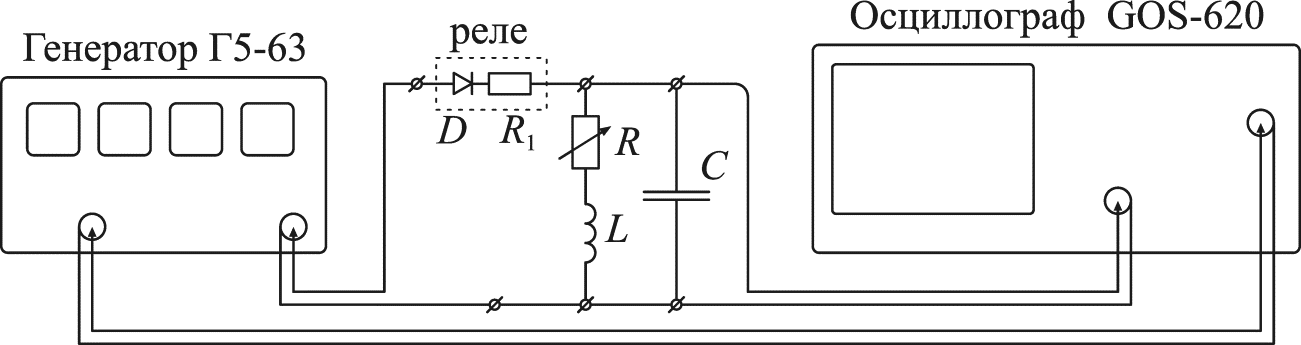
\includegraphics[width=0.7\linewidth]{curcuit.png}
\end{center}

\section{Задачи}
\begin{enumerate}
\item измерить периоды колебаний при нулевом сопротивлении реостата, проверить формулу $T = 2 \pi \sqrt{LC}$
\item выбрав конкретный конденсатор, подобрать с помощью реостата критическое сопротивление для данного контура
\item для этого конденсатора измерить добротность колебаний для разных сопротивлений с помощью амплитуд на пиках затухающей синусоиды
\item то же самое, только в XY-режиме осциллографа.
\item измерив сопротивление и индуктивность катушки, прикинуть добротность контура по формуле $Q = \frac{1}{R} \sqrt{\frac{L}{C}}$
\item сравнить значения добротности, полученные разными способами, проанализировать возможные расхождения
\end{enumerate}

\section{Результаты}
Значения емкостей конденсаторов измерены в методичке правильно, я проверил.
Катушку использовал на 400 витков.
\begin{tabular}{|c|}
ёмкость, нФ & период, мкс
21.86       & 77
33.23       & 92
50.72       & 110
70.83       & 130
100.3       & 160
223.6       & 240
477.5       & 340
927.7       & 480
\end{tabular}

\section{Выводы}

\end{document}
